\subsection{\acrshort{sift}}\label{sec:sift_stats}
\begin{figure}[H]
\begin{subfigure}[t]{0.45\linewidth}
    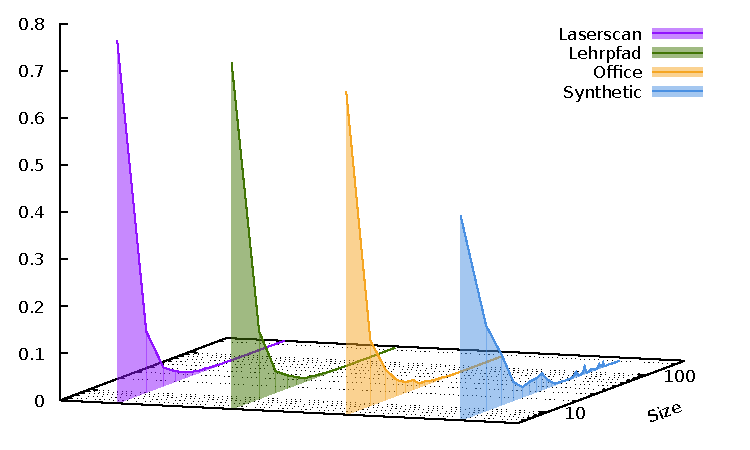
\includegraphics[width=\linewidth]{chapter06/results/SIFT/flexion/size.pdf}%
    \caption{\gls{flexion-image}}
\end{subfigure}\quad
\begin{subfigure}[t]{0.45\linewidth}
    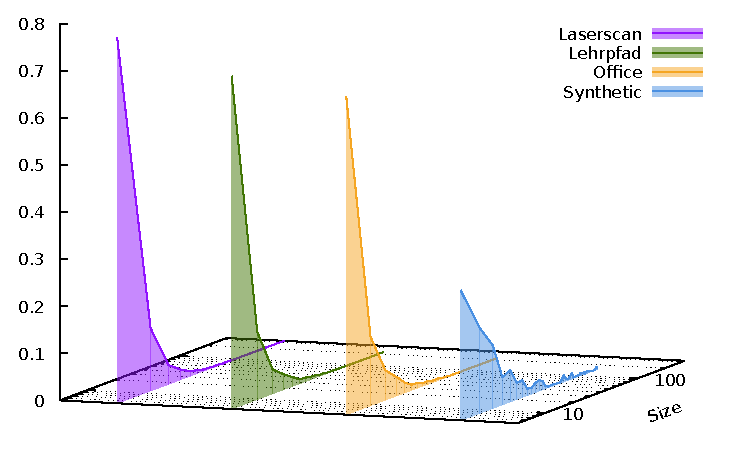
\includegraphics[width=\linewidth]{chapter06/results/SIFT/bearing/size.pdf}
    \caption{\gls{bearing-angle-image}}
\end{subfigure}\\
\begin{subfigure}[t]{0.45\linewidth}
    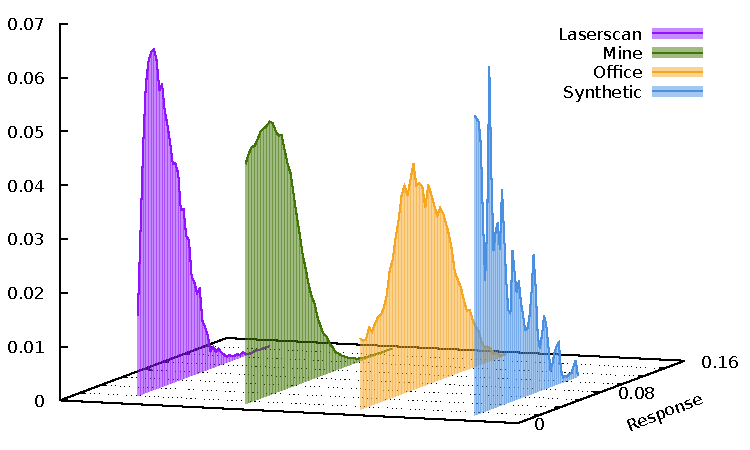
\includegraphics[width=\linewidth]{chapter06/results/SIFT/flexion/response.pdf}%
    \caption{\gls{flexion-image}}
\end{subfigure}\quad
\begin{subfigure}[t]{0.45\linewidth}
    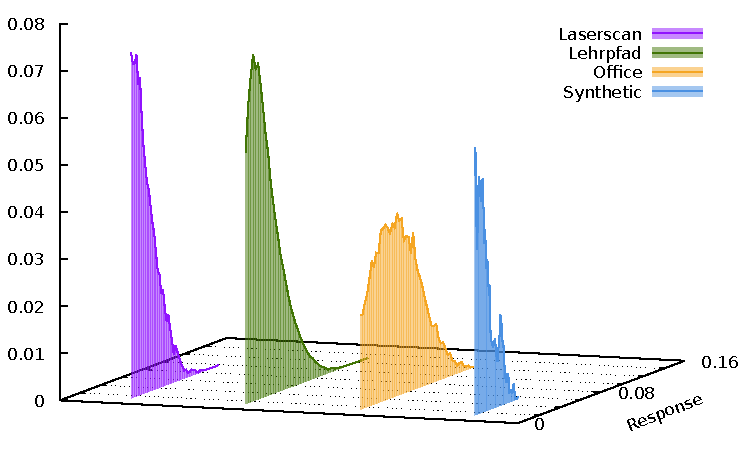
\includegraphics[width=\linewidth]{chapter06/results/SIFT/bearing/response.pdf}
    \caption{\gls{bearing-angle-image}}
\end{subfigure}
    \caption{Overview of keypoint sizes and responses for the \acrshort{sift} detector.}
\end{figure}
\begin{figure}[H]
    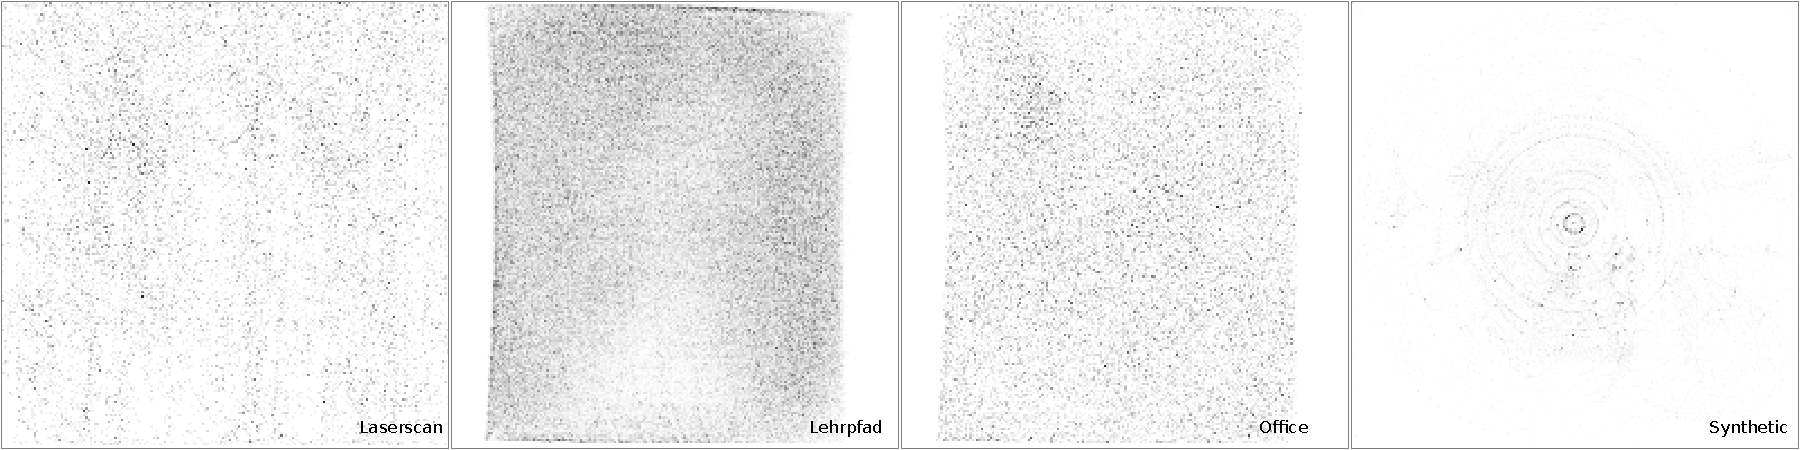
\includegraphics[width=\linewidth]{chapter06/results/SIFT/flexion/distribution.pdf}\\
    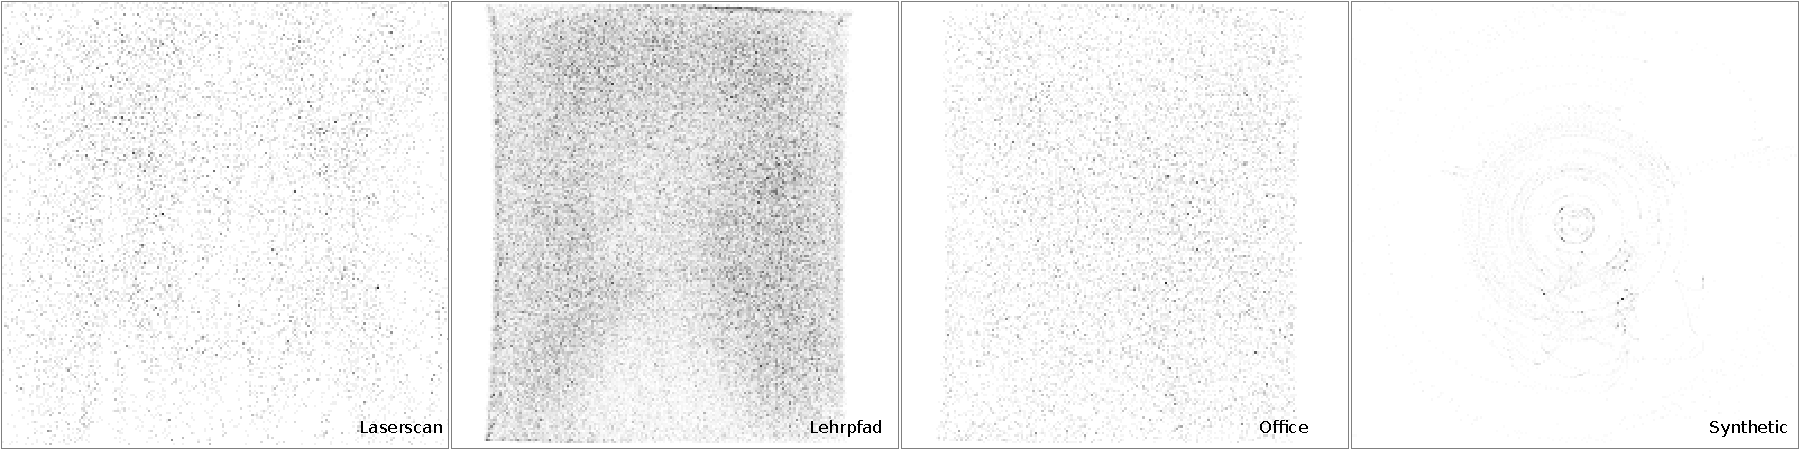
\includegraphics[width=\linewidth]{chapter06/results/SIFT/bearing/distribution.pdf}%
    \caption{Keypoint distribution for the \acrshort{sift} detector.}\label{fig:sift_kp_distribution}
\end{figure}
